\documentclass[a4paper,12pt]{article}
\usepackage[polish]{babel}
\usepackage[utf8]{inputenc}
\usepackage[T1]{fontenc}
\usepackage{latexsym}
\usepackage{graphicx}
\usepackage{fancyhdr}
\usepackage{chngpage}
\usepackage{enumerate}
\usepackage{enumitem}
\usepackage{listings}
\usepackage{geometry}
\linespread{1.5}
\pagestyle{fancy}
\geometry{lmargin=3.5cm, rmargin=2.5cm, bmargin=3cm, tmargin=3cm}

\lhead{}

\title
{
	\Large
	Akademia Górniczo-Hutnicza im. Stanisława Staszica \\ w Krakowie \\
	\vspace{10 mm}
	
\includegraphics[scale=0.8]{gfx/agh.jpg} \\
	\textbf{ System wykrywania podobieństw kodów źródłowych w projektach studenckich } \\
	Praca dyplomowa \\
	\vspace{10 mm}
}
\author
{
	\vspace{10 mm}
	Jarosław Szczęśniak \\
	Promotor: dr inż. Darin Nikolow
	\vspace{10 mm}
}

\begin{document}

\maketitle

\pagebreak

\tableofcontents

\newpage

\section{Wstęp}

\section{Cel i zakres prac}

Celem pracy jest zbudowanie systemu, który będzie wspomagał wykrywanie podobieństw w danych kodach źródłowych. Docelowym zagadnieniem z jakim ma zmierzyć się system jest porównywanie kodów źródłowych napisanych w języku Asembler.

Osiągnięcie celu głównego wymaga zrealizowania szeregu celów cząstkowych:
\begin{itemize}
\item zapoznanie się z dostępnymi metodami porównywania tekstu
\item zdefiniowanie języka wewnętrznego:
\begin{itemize}
	\item symboli leksykalnych
	\item gramatyki języka
	\item akcji semantycznych
\end{itemize}
\item implementacja co najmniej jednej metody porównywania
\item dostarczenie aplikacji analizującej kod źródłowy
\item dostarczenie środowiska do porównywania kodów źródłowych
\item dostarczenie przykładowych programów w języku wewnętrznym
\end{itemize}
	
Pierwszym etapem całego mechanizmu powinien być etap preprocessingu, czyli odpowiedniego przefiltrowania plików źródłowych, celem usunięcia zbędnych białych znaków oraz komentarzy.

Następnym krokiem jest proces analizy leksykalnej, którego zadaniem jest wyłonienie odpowiednich symboli leksykalnych, które zostaną przekazane do analizatora składniowego.

Kolejnym krokiem jest parsowanie, które odbywa się za pomocą analizatora składniowego. Sprawdza on, czy przekazane symbole wejściowe są zgodne z gramatyką języka oraz buduje z nich tzw. drzewo składniowe, które będzie wykorzystywane podczas porównywania dwóch kodów źródłowych.

Istnieje kilka skutecznych metod porównywania tekstu, poczynając od najprostszej i zarazem najmniej efektywnej metody brute-force, poprzez szybsze funkcje wykorzystujące zróżnicowane metody (np. funkcje hashujące), do algorytmów wykorzystujących deterministyczne automaty skończone.

Etap analizy można podzielić na 3 elementarne części:
\begin{itemize}
\item analizę leksykalną – wczytywanie znaków i grupowanie ich w większe symbole
\item analizę składniową – sprawdzenie poprawności z gramatyką, stworzenie drzewa składniowego
\item analizę semantyczną – analizę kodu na podstawie drzewa składniowego, zapewnienie odpowiednich warunków (zgodność typów, wywoływanie odpowiednich funkcji, sprawdzanie zasięgów)
\end{itemize}

Założenia co do funkcjonalności języka wewnętrznego:
\begin{itemize}
\item obsługa mechanizmu tworzenia zmiennych
\item obsługa pętli
\item obsługa instrukcji warunkowych
\item sprawdzanie wywoływanych funkcji
\item mechanizmu obsługi wywoływanych funkcji (ilość przekazywanych parametrów, zwykłe oraz rekurencyjne wywoływanie funkcji)
\end{itemize}
	
Wynikiem tego etapu będzie łatwa do porównania lista symboli w postaci <function, value>, <variable, value>.

\newpage

\section{Teoria kompilacji}

Kompilator to program, który tłumaczy kod źródłowy na kod wynikowy. Składa się on z dwóch głównych etapów - analizy i syntezy.

Etap analizy składa się z trzech etapów pośrednich - analizy leksykalnej, składniowej i semantycznej. Polega on na rozłożeniu kodu źródłowego na czynniki składowe oraz na budowie jego reprezentacji pośredniej.

Ten właśnie etap wydaje się być odpowiednim procesem, dzięki któremu można będzie wykonać porównanie dwóch kodów źródłowych na odpowiednio niskim poziomie, aby uniezależnić się od wykorzystywanego nazewnictwa lub organizacji i kolejności instrukcji w kodach źródłowych.


Język formalny to podzbiór zbioru wszystkich wyrazów nad skończonym alfabetem. Język formalny jest podstawowym pojęciem w informatyce, logice matematycznej i językoznawstwie. Aby zdefiniować język formalny musimy najpierw zdefiniować jego alfabet, składający się z symboli. Ciągi symboli nazywamy napisami, a dowolny zbiór tych ciągów to język formalny.

\subsection{Symbole}

Symbole leksykalne to abstrakcyjne  ciągi znaków, które definiowane są podstawie określonych przez analizator reguł i przekazywane do dalszych etapów analizy. Reguły, według których są one definiowane, budowane są najczęściej z wyrażeń regularnych.  Z symbolami leksykalnymi skojarzona jest też wartość leksykalna.
\\ \\
<przyklad> \\
sum = 3 + 2 ; \\
symbol 			| 	wartość \\
identyfikator		| 	sum \\
operator przypisania	|	= \\
liczba			|	3 \\
operator dodawania	|	+ \\
liczba			|	2 \\
koniec operacji		|	; \\
</przyklad> \\

Symbole, których używany najczęściej to litery lub cyfry. Alfabet jest to niepusty zbiór, składający się ze skończonej liczby symboli. Przykładem alfabetu, może być alfabet języka polskiego lub alfabet Morse’a.

Napis jest to skończony ciąg symboli, które należą do podanego alfabetu. Długość napisu oznaczamy jako |n| i jest to ilość symboli w napisie ,,n’’, przykładowo długość |tekst| wynosi 5.

Prefiksem napisu nazywamy pewną liczbę symboli rozpoczynających napis. Sufiksem nazywamy pewną liczbę symboli kończących napis. 

Język jest dowolnym zbiorem napisów ustalonym nad pewnym okreśłonym alfabetem. Językiem może być zbiór pusty, zbiór zawierający pusty napis lub pewien podzbiór ze zbioru wszystkich łańcuchów nad określonym alfabetem.

\subsection{Wyrażenia regularne}

\subsection{Gramatyka}

To, co definiuje leksemy, to zestaw reguł określonych na podstawie specyfikacji języka programowania, czyli gramatyki.

Obecnie najczęściej stosuje się wyrażenia regularne do zdefiniowania reguł. Określają one zestaw możliwych sekwencji, które są użyte do zbudowania konkretnych leksemów.

W niektórych językach programowania kod dzieli się na bloki za pomocą par symboli (np. ,,\{‘’ i ,,\}’’), które razem z wszelkimi białymi znakami również opisane są za pomocą leksemów, lecz nie są brane pod uwagę podczas dalszych etapów analizy.

\subsection{Analiza leksykalna}

Analiza leksykalna służy do dzielenia strumienia znaków wejściowych na grupy (symbole), do których dopasowywane są pewne sekwencje (leksemy) na podstawie reguł (wzorców), w celu przekazania ich do dalszego etapu analizy. Leksem to abstrakcyjna jednostka leksykalna, która może obejmować słowa kluczowe, identyfikatory, etykiety, operatory, separatory, komentarze lub inne symbole specjalne.

\subsubsection{Skaner}

Skaner, czyli podstawowa część analizatora leksykalnego, zajmuje się głównym etapem analizy. Posiada on informacje na temat sekwencji znaków, które mogą być wykryte i zapisane jako symbole.

W wielu przypadkach pierwszy znak, który nie jest znakiem białym może posłużyć do dedukcji, z jakiego rodzaju symbolem mamy do czynienia (longest-match rule). W przypadku bardziej skomplikowanych języków potrzebna jest możliwość cofania się do wcześniej wczytanych znaków.

Skaner wczytuje kolejne znaki ze strumienia wejściowego i klasyfikuje je według reguł w symbole leksykalne, które następnie przekazywane są do analizy składniowej. Jako jednostka rozpoczynająca analizę i wczytująca tekst źródłowy może służyć również jako filtr, który pomija pewne elementy, takie jak np. komentarze, białe znaki lub znaki nowego wiersza.


Możliwe jest i czasem konieczne napisanie własnego analizatora, aczkolwiek jest to zwykle zbyt skomplikowane, czasochłonne i nieopłacalne. Z tego względu analizatory, zwane lekserami, zwykle generowane są za pomocą specjalnych narzędzi, które przyjmują na wejściu wyrażenia regularne, które opisuję wymagane symbole leksykalne.

\subsection{Analiza składniowa}

Analiza składniowa to proces analizy tekstu, złożonego z symboli, którego celem jest wyklarowanie jego struktury gramatycznej na podstawie zdefiniowanej gramatyki.

\subsubsection{Parser}

Jest to komponent, który wykonując analizę składniową, sprawdza jej poprawność i tworzy pewną strukturę danych (często tzw. drzewo składniowe), składającą się z symboli wejściowych. Korzysta z analizatora leksykalnego, który zaopatruje go w zestaw symboli leksykalnych zbudowanych ze strumienia wejściowego. Innymi słowy parser analizuje kod źródłowy i tworzy jego wewnętrzną reprezentację.

\subsubsection{Typy parserów}

Zadaniem parsera jest określenie czy i w jaki sposób symbole leksykalne mogą być przekształcone na symbole gramatyczne. Istnieją dwa sposoby, dzięki którym osiągniemy rządany efekt:
\begin{itemize}
	\item parsowanie zstępujące (top-down) -- polega na znalezieniu symboli wysuniętych najbardziej na lewo przeszukując drzewo składniowe z góry na dół.
	\item parsowanie wstępujące (bottom-up) -- polega na sprawdzeniu począwszy od słowa wejściowego i próbie redukcji do symbolu startowego, analizę zaczynamy od liści drzewa posuwając się wkierunku korzenia.
\end{itemize}

\subsection{Opis procesu}

%\section{Analiza semantyczna}

\newpage

\section{Metody porównywania}

Każda z opisanych metod posiada szereg cech ją charakteryzujących. Są to:
\begin{itemize}
\item faza preprocesingu - przygotowania danych wejściowych do analizy
\item ilość potrzebnej pamięci dodatkowej
\item złożoność czasowa - ilość wykonywanych operacji względem ilości danych wejściowych
\end{itemize}

\subsection{Algorytm brute-force}

Metoda brute -- force, w teorii, jest najskuteczniejszą metodą, ponieważ sukcesywnie sprawdza wszystkie możliwe kombinacje w poszukiwaniu rozwiązania problemu. W praktyce jednak, algorytmy oparte na tej metodzie są niezwykle nieoptymalne, ze względu na czas wykonywania, przez co są rzadko stosowane.

Algorytm polega na sprawdzeniu wszystkich pozycji w tekscie pomiędzy znakiem $0$ i $n-m$, gdzie $m$ to długość poszukiwanego wzorca, a $n$ to długość tekstu. Algorytm weryfikuje, czy wzorzec zaczyna się na danej pozycji. Jeśli tak to pozycja elementu w tekscie zapisywana jest do bufora. Następnie przesuwa wskaźnik w prawo po każdej próbie. Jeśli na kolejnych pozycjach znajdują się wszystkie kolejne elementy z wzorca to do tablicy wynikowej przepisywany jest zawartość bufora. Algorytm może być wykonywany w dowolnym kierunku, od przodu lub od tyłu.

Metoda nie wymaga żadnej fazy przed rozpoczęciem wykonywania algorytmu. Ze względu na charakter metody wymaga dodatkowego miejsca w pamięci. Złożoność czasowa wynosi $O(m*n)$, a ilość operacji potrzebna do wykonania algorytmu wynosi $2n$.

Przykładowy kod źródłowy algorytmu brute -- force, wyszukującego określony wzorzec w podanym tekście:
\begin{lstlisting}
void BF(char *x, int m, char *y, int n) {
   int i, j;
   for (j = 0; j <= n - m; ++j) {
      for (i = 0; i < m && x[i] == y[i + j]; ++i);
      if (i >= m)
         OUTPUT(j);
   }
}
\end{lstlisting}

\subsection{Deterministyczny automat skończony}

DFA (Deterministic Finite Automaton), czyli deterministyczny automat skończony to maszyna o skończonej liczbie stanów, która czytając kolejne symbole podanego słowa zmienia swój stan na wartość funkcji opisującej dany symbol. Po przeczytaniu całego słowa automat sprawdza, czy znajduję się w jednym z określonych stanów akceptacyjnych.

Algorytm zbudowany na podstawie DFA na początku wymaga stworzenia minimalnego skończonego automaty $A(x)$ rozpoznającego język $\sum_{}^*x$, w celu znalezienia słowa $x$. Minimalny automat określony wzorem $A(x)=(Q, q_0, T, E)$ rozpoznający język $\sum_{}^*x$ definiujemy następująco:
\begin{itemize}
\item $Q$ to zbiór wszystkich przedrostków słowa $x$: \\
$Q = \{ \epsilon , x[0], x[0..1], .. , x[0..m-2] \} $, gdzie $ \ epsilon $ -- zbiór pusty
\item $q_0 = \epsilon $
\item $T = \{ x \} $
\item dla $q$ należącego do $Q$ ($q$ to przedrostek $x$) i $a$ w $\sum_{}$ $(q, a, qa)$ należy do $\sum_{}$ wtedy i tylko wtedy, gdy $qa$ jest także przedrostkiem słowa $x$, w przeciwnym razie $(q, a, p)$ należy do $\sum_{}$, a $p$ jest najdłuższym przyrostkiem $qa$, który jest przedrostkiem słowa $x$
\end{itemize}

Po stworzeniu DFA przeszukiwanie słowa $x$ w tekście $y$ polega na przeanalizowaniu tekstu $y$ przez DFA rozpoczynając ze stanem $q_0$. Za każdym razem, gdy trafiono na terminal ($T$ - szukane słowo) raportowane jest wystąpienie szukanego słowa.

Stworzenie DFA $A(x)$ ma złożoność czasową rzędu $O(m+\sigma)$ i potrzebuje $O(m\sigma)$ miejsca, natomiast sam etap przeszukiwania ma złożoność czasową $O(n)$.

Przykładowa implementacja DFA:
\begin{lstlisting}
void preAut(char *x, int m, Graph aut) {
   int i, state, target, oldTarget;
   for (state = getInitial(aut), i = 0; i < m; ++i) {
      oldTarget = getTarget(aut, state, x[i]);
      target = newVertex(aut);
      setTarget(aut, state, x[i], target);
      copyVertex(aut, target, oldTarget);
      state = target;
   }
   setTerminal(aut, state);
}
 
void AUT(char *x, int m, char *y, int n) {
   int j, state;
   Graph aut;
   /* Preprocessing */
   aut = newAutomaton(m + 1, (m + 1)*ASIZE);
   preAut(x, m, aut);
   /* Searching */
   for (state = getInitial(aut), j = 0; j < n; ++j) {
      state = getTarget(aut, state, y[j]);
      if (isTerminal(aut, state))
         OUTPUT(j - m + 1);
   }
}
\end{lstlisting}

\newpage

\subsection{Algorytm Karp-Rabin}

Algorytm Karpa-Rabina jest kolejnym algorytmem służącym do przeszukiwania określonego podciągu w tekście. Algorytm ten korzysta z funkcji hashującej, co jest prostą metodą, aby w większości przypadków uniknąć kwadratowej liczby porównań znakowych. Zamiast sprawdzania znaku na każdej pozycji tekstu, w celu odnalezienia wzorca, bardziej wydajne jest sprawdzenie, czy zawartość “okna” przypomina wzorzec. Sprawdzanie podobieństwa pomiędzy wzorcem i “oknem” odbywa się za pomocą funkcji hashującej.
\\ \\
Właściwości funkcji hashującej:
\begin{itemize}
\item Wydajność obliczeń
\item Dyskryminuje słowa
\item funkcja $hash(y[j+1 .. j+m])$ musi być łatwo przeliczalna z $hash(y[j .. j+m-1])$ oraz $y[j+m]$: \\
$hash(y[j+1 .. j+m]) = rehash(y[j], y[j+m], hash(y[j .. j+m-1])$
\end{itemize}

Dla słowa $w$ o długości $m$ niech funkcja $hash$ będzie zdefiniowana następująco:
\begin{center}
$hash(w[0 .. m-1]) = (w[0]*2^{m-2} + ... + w[m-1]*2^0)mod(q)$, \\ gdzie $q$ jest dowolną dużą liczbą
\end{center}

Wtedy funkcja rehash przyjmuje postać:
\begin{center}
$rehash(a,b,h) = ((h-a*2^{m-2})*2+b)mod(q)$
\end{center}

Preprocessing - obliczenie funkcji hashującej dla szukanego wzorca - posiada złożoność czasową rzędu $O(m), gdzie m - długość wzorca.$

Podczas wyszukiwania wystarczy porównać $hash(x)$ z $hash(y[j .. j+m-1])$ dla $0 <= j <= n-m$. Jeśli równość jest znaleziona to należy sprawdzić równość $x = y[j .. j+m-1]$ znak po znaku.
\newpage
Przykład implementacji:
\begin{lstlisting}
#define REHASH(a, b, h) ((((h) - (a)*d) << 1) + (b))

void KR(char *x, int m, char *y, int n) {
   int d, hx, hy, i, j;

   /* Preprocessing */
   /* computes d = 2^(m-1) with
      the left-shift operator */
   for (d = i = 1; i < m; ++i)
      d = (d<<1);

   for (hy = hx = i = 0; i < m; ++i) {
      hx = ((hx<<1) + x[i]);
      hy = ((hy<<1) + y[i]);
   }

   /* Searching */
   j = 0;
   while (j <= n-m) {
      if (hx == hy && memcmp(x, y + j, m) == 0)
         OUTPUT(j);
      hy = REHASH(y[j], y[j + m], hy);
      ++j;
   }

}
\end{lstlisting}

\subsection{Algorytm Boyer-Moore}

Algorytm Boyer-Moore został stworzony w 1977 roku i do tej pory uważany jest za najbardziej optymalny algorytm poszukiwania wzorca w tekscie. Dowodem na to jest fakt, że algorytm ten jest zaimplementowany w większości najbardziej popularnych aplikacji z opcją ,,Znajdź’’ lub ,,Zamień’’.

Algorytm szuka danego wzorca w teksćie porównując kolejne znaki tekstu do wzorca, lecz w odróżnieniu od metody brute-force wykorzystuje informacje zebrane za pomocą fukcji preprocesujących, aby pominąć jak najwięcej znaków w tekście, które na pewno nie pasują do wzorca.

Procedura zaczyna się w miejscu k = n, w taki sposób, że początek wzorca P jest wyrównany do początku tekstu T. Następnie poszczególne znaki z P i T są porównywane począwszy od indeksu n w P i indeksu k w T, porusząjąc się od prawej do lewej strony wzorca P. Porównywanie trwa dopóki znaki w P i T nie są różne lub do momentu dotarcia do początku P (co oznacza, że znaleziono wystąpienie w tekście), a następnie indeks porównywania przesuwany jest w prawo o maksymalną wartość wskazywaną przez zdefiniowane reguły. Czynności są powtarzane do momentu sprawdzenia całego tekstu T.

Reguły przesuwania indeksu definiowane są za pomocą tabel tworzonych za pomocą funkcji preprocesujących.

Przykład implementacji:
\begin{lstlisting}
public List<Integer> match() {
	List<Integer> matches = new LinkedList<Integer>();
	computeLast();
	computeMatch();

	int i = text.length() - 1;
	int j = pattern.length() - 1;
	while (i >= 0 && i < text.length()) {
		try {
			if (pattern.charAt(j) == text.charAt(i)) {
				if (j == 0) {
					matches.add(i);
					j = pattern.length() - 1;
					// return i;
				}
				j--; i--;
			} else {
				i -= Math.max(match[j], last[text.charAt(i)] - text.length() + 1 + i);
				j = pattern.length() - 1;
			}
		} catch (Exception ex) { (...)  }
	}
	return matches;
}
\end{lstlisting}

\section{Wprowadzenie do Asemblera}

\section{Projekt systemu CodeComp}

W tym rozdziale przedstawiono opis aplikacji CodeComp, jej budowę wewnętrzną oraz sposoby instalacji i użycia.

\subsection{Architektura systemu}

Program składa się z czterech głownych pakietów: Comparator, Algorithm, Analyzer oraz GUI.

\begin{figure}[!h]
\centering
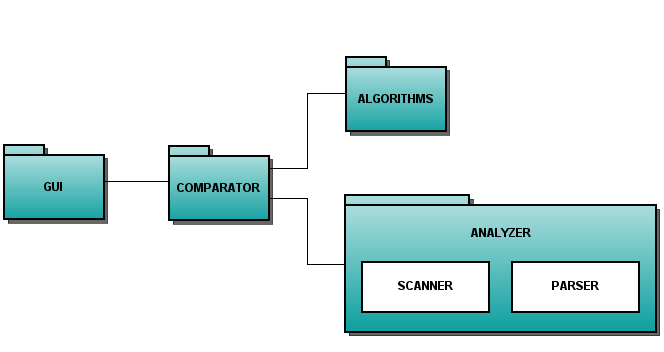
\includegraphics[scale=0.6]{gfx/packagediagram.png}
\end{figure}

Comparator jest podstawowym, statycznym obiektem, który na wejście pobiera kody źrodłowe programów wejściowych, uruchamia wybrany sposób porównywania i zwraca listę elementów podobnych oraz ich położenia w tekście.

Algorithm to pakiet, w którego skład wchodzi zestaw algorytmów porównywania tekstu. Użytkownik jest w stanie wybrać sobie wybrany algorytm w zależności od potrzeb, aby móc porównać jego skuteczność oraz czas działania.

Analyzer to komponent, który zajmuje się etapem analizy z teorii kompilacji. Składa się ze skanera - czyli analizatora leksykalnego - oraz z parsera - czyli analizatora składniowego. Wynikiem działania analizatora jest drzewo składniowe, które następnie będzie porównywane przez komparator.

\begin{figure}[!]
\centering
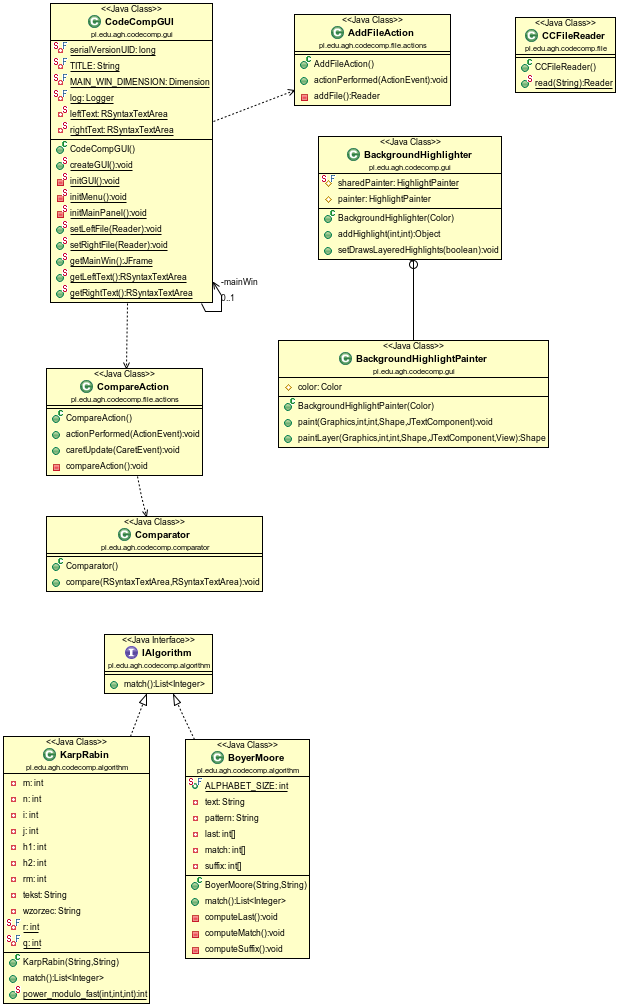
\includegraphics[scale=0.6]{gfx/classdiagram.png}
\end{figure}

\pagebreak

Program posiada graficzny interfejs użytkownika stworzony za pomocą bilbioteki Swing. Składa się on z dwóch elementów tekstowych wyświetlających wczytane kody źródłowe oraz podświetlający elementy, które są identyczne/podobne. Wczytywanie oraz wszelkie inne operacje dostępne są z poziomu głównego menu znajdującego się na górze okna.

\begin{figure}[!h]
\centering
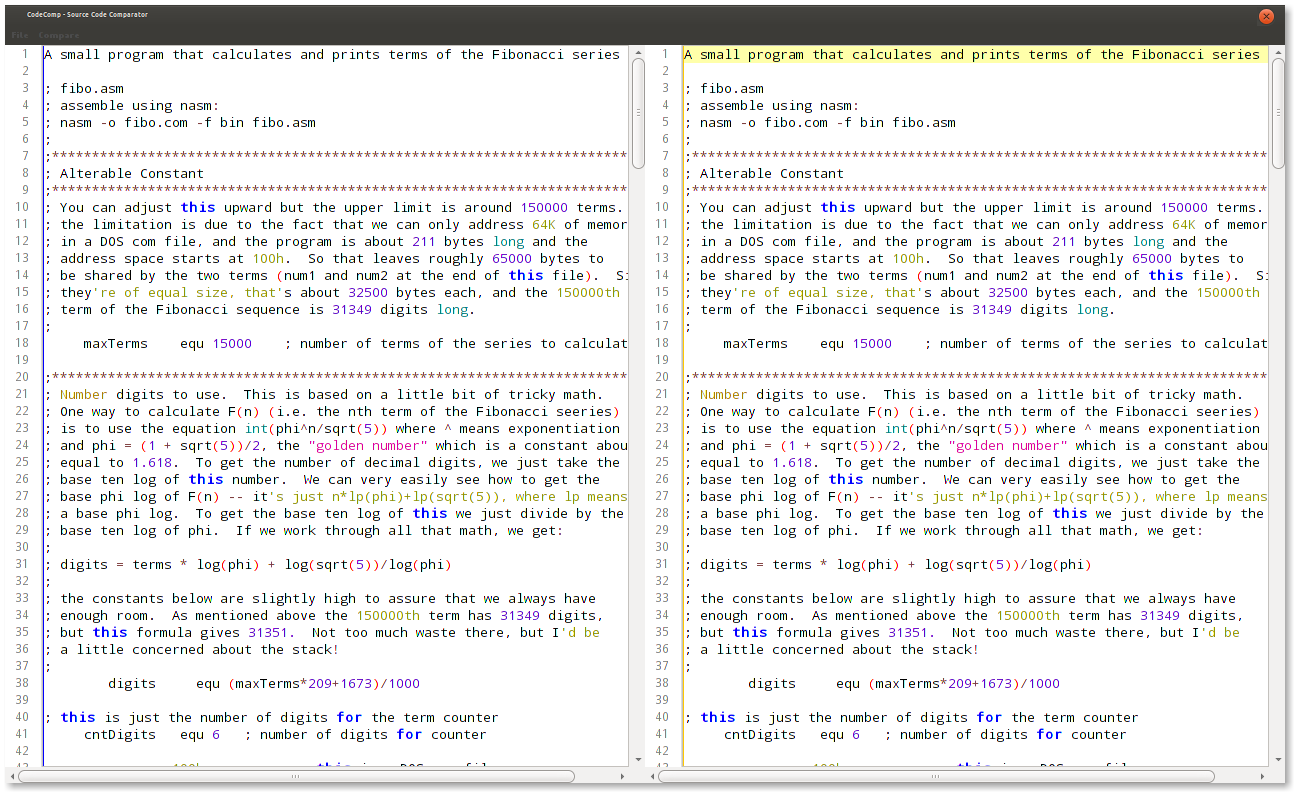
\includegraphics[scale=0.33]{gfx/main_window.png}
\end{figure}

\newpage

\subsection{Uruchamianie aplikacji}

Aplikacja dołączona do niniejszej pracy dyplomowej w całości napisana została w języku JAVA. Wykorzystuje ona podstawowe pakiety ze środowiska JRE 1.7 oraz kilka dodatkowych, niestandardowych bibliotek (rsyntaxtextarea).
\\ \\
Aplikacja dołączona została w postaci kodu źrodłowego oraz skompilowanego archiwum JAR, który można uruchomić na dowolnym środowisku z zainstalowanym pakietem uruchomieniowym JRE w wersji 1.7 za pomocą polecenia:
\\ \\
java -jar codecomp.jar

\subsection{Korzystanie z aplikacji}

\subsection{Wyniki}

\section{Wnioski}

\newpage

\section{Bibliografia}

\begin{thebibliography}{1}

\bibitem{temp} ldots

\end{thebibliography}

\end{document}
